% Tesis ITAM CLASS -- version 0.1 (13 - Abr - 2015)
% Clase para las tesis del ITAM
% 
% 13 - Abr - 2015 	Victor Martinez 	victor.martinez (at) itam.mx
% LICENSE: Creative Commons SA-BY 3.0
%
%
% Este documento presenta un ejemplo de uso de la plantilla
% El estudiante es libre de modificar este archivo a su gusto
% 
\documentclass{tesisITAM}
\usepackage[utf8]{inputenc}

\title{Generación automática de Lenguaje Natural a partir de Técnicas de Aprendizaje de Máquina}

\author{\textbf{DANAE SÁNCHEZ VILLEGAS}}
\degree{\textbf{INGENIERO EN COMPUTACIÓN}}
\advisor{DR. CARLOS FERNANDO ESPPONDA DARLINGTON}
\year{2016}

\begin{document}

	\pagenumbering{gobble}
	\maketitle
	\publicationrights

	%%%%%%%%%%%%%%%%%%%%%%%%%%%%%%%%%%%%%%%%%%%%%%
	% ABSTRACT
	%%%%%%%%%%%%%%%%%%%%%%%%%%%%%%%%%%%%%%%%%%%%%%

	\begin{abstract}{spanish}
		Este documento presenta una plantilla para usar en las tesis y tesinas del ITAM. Se provee de manera gratuita y sin ninguna responsabilidad bajo la licencia \emph{creative commons BY-SA 3.0}.
	\end{abstract}

	\begin{abstract}{english}
		In this work we present a template for thesis and titulation works presented at ITAM. It is provided freely and without any responsability under the \emph{creative commons BY-SA 3.0}. 
	\end{abstract}


	\selectlanguage{english} 
	\setcounter{page}{1}
	\pagenumbering{roman}

	\tableofcontents
	\listoffigures
	\listoftables
	\newpage

	\pagenumbering{arabic}
	\setcounter{page}{1}

	%%%%%%%%%%%%%%%%%%%%%%%%%%%%%%%%%%%%%%%%%%%%%%
	% CONTENT
	%%%%%%%%%%%%%%%%%%%%%%%%%%%%%%%%%%%%%%%%%%%%%%
	 \chapter{Introduction}
\label{ch:intro}

\begin{chapterquote}{Leslie Lamport}
	Formal mathematics is nature's way of letting you know how sloppy
your mathematics is.
\end{chapterquote}

Este trabajo presenta una plantilla para las tesis y tesinas del Instituto Tecnológico Autónomo de México para los usuarios de \LaTeX \cite{lamport1994latex}. Nace de la necesidad de los matemáticos, actuarios e ingenieros (entre otras carreras) por utilizar un sistema de composición de textos adecuado para su trabajo de titulación. El objetivo es ayudar a la comunidad del ITAM a simplificar el proceso de escritura y edición de sus tesis, tesinas o casos. A continuación describimos a mayor detalle cada una de las partes de la plantilla.

\subsection{Natural Language Processing}
	\subsubsection{N-grams}
The standard approach to statistical modelling of language was based on counting frequencies of occurrences of short symbol sequences of length up to N (called N-grams). The number of possible N-grams is on the order of VN, where V is the vocabulary size N-grams treat each word as an atomic unit, so they cannot generalize across semantically related sequences of words, whereas neural language models can because they associate each word with a vector of real valued features, and semantically related words end up close to each other in that vector space (Fig. 4).\cite{lecun2015deep}

    \subsubsection{Prediction by Partial Matching}
The prediction by partial algorithms are compression algorithms where the prediction is determined by counting exact matches between the recent history and the training set \cite{graves2013generating}.
    
    \subsubsection{Neural Language Models}
Before the introduction of neural language model the standard approach to statistical modelling of language did not exploit distributed representations\cite{lecun2015deep}

\subsection{Machine Learning}

\subsection{Neural Networks}
After training, the performance of the system is measured on a different set of examples called a test set. This serves to test the generalization ability of the machine\cite{lecun2015deep}.
\subsubsection{Backpropagation}
	The weight vector is formed by the internal adjustable parameters which are adjusted to reduce the distance between the output scores and the desired pattern of the scores. To adjust the weight vector, for each weight, indicates by what amount the error would increase or decrease if the weight were increased by a tiny amount. The weight vector is then adjusted in the opposite direction to the gradient vector\cite{lecun2015deep}.

it was commonly thought that simple gradient descent would get trapped in poor local
minima In practice, poor local minima are rarely a problem with large networks.\cite{lecun2015deep}



\subsection{Deep Learning}
Representation learning is a set of methods that allows a machine to be fed with raw data and to automatically discover the representations needed for detection or classification. Deep-learning methods are representation-learning methods with multiple levels of representation. With the composition of enough such transformations, very complex functions can be learned. For classification tasks, higher layers of representation amplify aspects of the input that are important for discrimination and suppress irrelevant variations\cite{lecun2015deep}.


\subsection{Recurrent Neural Networks}
A recurrent neural network is a artificial neural network model.The difference of its structure is that connections among hidden units associated with a time delay are allowed, enabling the model to retain information about the past inputs. In this way, temporal correlations between events that are possibly far away from each other in the data can be discovered \cite{pascanu2013difficulty}. 

The network is `deep' in both space and time, in the sense that every piece of information passing either vertically or horizontally through the computation graph will be acted on by multiple successive weight matrices and nonlinearities \cite{graves2013generating}.

RNNs are fuzzy in the sense that they use their internal representation to perform a high-dimensional interpolation between training examples so they do not use exact temples from the training data to make predictions \cite{graves2013generating}
The result is that rnns synthesise and reconstitute the training data in a complex way, and rarely generate the same thing twice. Furthermore, fuzzy predictions do not suffer from the curse of dimensionality, and are therefore much better at modelling real-valued or multivariate data than exact matches  \cite{graves2013generating}.

For tasks that involve sequential inputs, such as speech and language, it results better to use RNNs. RNNs process an input sequence one element at a time, maintaining in their hidden units a ‘state vector’ that implicitly contains information about the history of all the past elements of the sequence.\cite{lecun2015deep}


\subsubsection{Backpropagation Through Time}

RNNs, once unfolded in time (Fig. 5), can be seen as very deep feedforward networks in which all the layers share the same weights\cite{lecun2015deep}
One approach to compute the gradients is Backpropagation Through Time (BPTT). Here, the model is presented as a deep multi-layer one where backpropagation is applied on the unrolled model\cite{pascanu2013difficulty}.
The backpropagation procedure to compute the gradient of an objective function with respect to the weights of a multilayer stack of modules is nothing more than a practical application of the chain rule for derivatives. The key insight is that the derivative (or gradient)
of the objective with respect to the input of a module can be computed by working backwards from the gradient with respect to the output of that module (or the input of the subsequent module). The backpropagation equation can be applied repeatedly to propagate gradients through all modules, starting from the output at the top (where the network produces its prediction) all the way to the bottom (where the external input is fed). Once these gradients have been computed, it is straightforward to compute the gradients with respect to the weights of each module. To go from one layer to the next, a set of units compute a weighted sum of their inputs from the previous layer and pass the result through a non-linear function \cite{lecun2015deep}

\subsubsection{RNS Training Issues}
RNNs are very powerful dynamic systems, but training them has proved to be problematic because the backpropagated gradients either grow or shrink at each time step, so over many time steps they typically explode or vanish\cite{lecun2015deep}

The exploding gradients problem refers to the large increase in the norm of the gradient during training caused by the explosion of the long term components. On the other hand, the vanishing gradients problem is presented when long term components go exponentially fast to norm 0 making impossible for the model to learn correlation between temporally distant events \cite{pascanu2013difficulty}. 

\begin{enumerate}
\item The exploding gradients problem \\
 One simple mechanism to deal with the exploding gradients problem is to rescale them whenever they go over a threshold. One good heuristic for setting this threshold is to look at statistics on the average norm over a sufficiently large number of updates. In this way, we can handle very abrupt changes in norm, so the algorithm can be thought of as adapting the learning rate based on the norm of the gradient  \cite{pascanu2013difficulty}.
Algorithm
\item The vanishing gradients problem \\
The vanshing gradients problem makes it difficult to learn to store information for very long. 
This amnesia makes them prone to instability when generating sequences. The problem is that if the network's predictions  are only based on the last few inputs, and these inputs were themselves predicted by the network, it has little opportunity to recover from past mistakes. Having a longer memory has a establishing effect, because even if the network cannot make sense of its recent history, it can look further back in the past to formulate its predictions. \cite{graves2013generating}

A solution proposed for the vanishing gradient problem is to use a regularization term that forces the error signal not to vanish as it travels back in time  write the algorithm 1 and the regularization term \cite{pascanu2013difficulty}.
A second idea is to augment the network with an explicit memory. The first proposal of this kind is the long short-term memory (LSTM) networks.

\end{enumerate}
\subsubsection{Long Short-Term Memory Networks}
Long Short-term Memory (LSTM) is an RNN architecture designed to be better at storing and accessing information than standard RNNs \cite{graves2013generating}.
Although in most RNNs the hidden layer function H is an elementwise application of sigmoid function.,  Long Short-Term Memory  architecture uses purpose-built memory cells to store information, is better at finding and exploiting long range dependencies in the data. It has a input gate, forget gate, output gate, cell and cell input activation vectors, all of which are the same size as the hidden vector h. \cite{graves2013generating}
The memory cell (hay que ver cual de las 3 es) acts like an accumulator or a gated leaky neuron: it has a connection to itself at the next time step that has a weight of one, so it copies its own real-valued state and accumulates the external signal, but this self-connection is multiplicatively gated by another unit that learns to decide when to clear the content of the memory \cite{lecun2015deep}.

LSTM networks have subsequently proved to be more effective than conventional RNNs, especially when they have several layers for each time step\cite{lecun2015deep}.
The full gradient can be calculated with backpropagation through time \cite{graves2013generating}
This model has been used in several applications such as speech and handwriting recognition.\cite{graves2013generating}



\section{Language Modelling}
Recurrent Neural Networks are dynamic models that have been used to generate sequences in different domains such as music, text and motion capture data \cite{graves2013generating}.
They also have been found to be very good at predicting the next character in the text or the next word in a sequence, since the hidden layers of a multilayer neural network learn to represent the network’s inputs in a way that makes it easy to predict the target outputs.\cite{lecun2015deep}

Novel sequences can be generated by by a trained network by iteratively sampling from the network's output distribution, assuming the predictions are probabilistic and then feeding in the sample as input at the next step, meaning by making the network treats its inventions as if they were real. 
\cite{graves2013generating}.


\subsection{Words Representation}
Text data is discrete, and is typically presented to neural networks using `onehot' input vectors. That is, if there are K text classes in total, and class k is fed in at time t, then xt is a length K vector whose entries are all zero except for the kth, which is one. Pr(xt+1jyt) is therefore a multinomial distribution, which can be naturally parameterised by a softmax function at the output layer:
formulas
\begin{enumerate}
\item Word-level language modelling \\
In most cases, text prediction  is performed at the word level. K is therefore the number of words in the dictionary. \cite{graves2013generating}
In the first layer, each word creates a different pattern of activations, or word vectors (Fig. 4). In a language model, the other layers of the network learn to convert the input word vectors into an output word vector for the predicted next word, which can be used to predict the probability for any word in the vocabulary. Learning word vectors turned out to also work very well when the word sequences come from a large corpus of real text and the individual micro-rules are unreliable.\cite{lecun2015deep}

This can be problematic for realistic tasks, where the number of words often exceeds 100,000. As well as requiring many parameters to model, having so many classes demands a huge amount of training data to adequately cover the possible contexts for the words. A further diculty is the high computational cost of evaluating all the exponentials during training. Furthermore, word-level models are not applicable to text data containing non-word strings, such as multi-digit numbers or web addresses.\cite{graves2013generating}

\item Character-level language modelling \\
Character-level language modelling has been found to give slightly worse performance than equivalent word-level models. Nonetheless, predicting one character at a time is more interesting from the perspective of sequence generation, because it allows the network to invent novel words and strings.
\cite{graves2013generating}


\end{enumerate}
	\chapter{Theoretical Framework}
\label{ch:teo}

\begin{chapterquote}{Herbert Simon}
Human beings, viewed as behaving systems, are quite simple.
The apparent complexity of our behavior over time is largely a
reflection of the complexity of the environment in which we find
ourselves.
\end{chapterquote}


\section{Machine Learning}

The process of learning has long fascinated people from many different disciplines such as psychology, biology, neuroscience, computer science, statistics, mathematics, physics, etc. However, it has been difficult to agree upon a precise definition of the process mainly because it depends on the viewpoint. When looking for the meaning of learning in the dictionary we can find: "acquire knowledge of something through study or experience", "conceiving something for mere appearances, or with little foundation", and "to fix something in memory"(RAE). Since this work is motivated on the desire to make computers learn like human beings, one immediate alternative would be a brain simulation. Unfortunately, brain simulation faces two main obstacles\cite{natarajan2014machine}:
\begin{enumerate}
\item  The detailed structure of the brain is not known yet
\item Even if we knew the detailed structure of the brain, it does not exist a fast enough computer to simulate it. 
\end{enumerate}

Thus, the focus would need to be less on the specific mechanisms that biological brains use to organize themselves and more on the study of a fast and effective organizational algorithm along with a set of conditions which allow to construct models that imitate a specific and limited behavior of humans\cite{strom2007hebbian}. In this case, the behavior is the generation of a natural language such as English or Spanish. Our main source for teaching a computer to learn this task is data, so the key concept to think is learning from data. And translated to human behavioral terms, this concept refers to learning from experience
%\cite{marsland2015machine}. 

Therefore, machine Learning is about making computers modify or adapt their actions so that these actions get more accurate, where accuracy is measured by how well the chosen actions reflect the correct ones. As there are several ways to achieve this task there are different types of machine learning explained as follows \cite{marsland2015machine}:

\begin{itemize}
\item \textbf{Supervised Learning} It is said that it is supervised learning when a training set of examples with the correct responses or targets are provided and, based on this training set, the algorithm generalises to respond correctly to all possible inputs.

\item \textbf{Unsupervised Learning} The algorithm tries to identify similarities between the inputs so that the inputs that have something in common are categorised together. In this type of learning correct responses are not provided.

\item \textbf{Reinforcement Learning} The algorithm gets told when the answer is wrong but does not get told how to correct it. Instead, it has to explore and try out different possibilities until it works out how to get the right answer. 

\item \textbf{Evolutionary learning} In this type of learning, biological evolution is seen as a learning process where the organisms adapt to improve their survival rates and chance of having offspring in their environment. It uses an idea of fitness which corresponds to a score for how good the solution is. 
\end{itemize}

\section{McCulloch and Pitts Neurons}
McCulloch and Pitts modeled an artificial neuron as a mathematical model in order to extract only the essentials required to accurately represent the entity, removing all the obscured details. They took in account three basic elements: a set of weighted inputs ($w_i$), an adder that sums the input signals, and an activation function that decides if the neuron fires to the current inputs.
\begin{figure}[h]
\centering
 
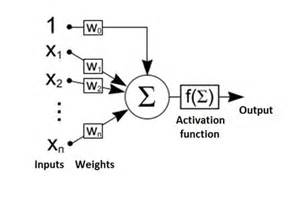
\includegraphics[width=10cm,height=5cm]{model_of_neuron.jpg}
\caption{McCulloch and Pitt's Neuron Model}
\label{fig:neuron}
\end{figure}

The signals are added and if the sum is greater than the threshold $\theta$ then, it is activated. The mathematical expression is as follows:\\
\begin{equation} \label{eq:neuron}
h=\sum_{i=1}^{m} w_i * x_i + b
\end{equation}\ref{eq:neuron}

Thus the output of the neuron is the sum of the $m$ inputs ($x_i$) multiplied by the weights ($w_i$). Furthermore, units can be given biases by introducing an extra input to each unit which always has a value of 1. The weight on this extra input is called the bias (b) and is equivalent to a threshold of the opposite sign \cite{polk2002cognitive}. 


\section{Neural Networks}

A simple neural network is shown in Figure \ref{fig:nn}. It is formed by input units at the bottom, any number of intermediate or hidden layers, and a layer of output units at the top. Each of the units are  defined as a McCulloch and Pitts neuron. It should be noticed that connections within a layer from a higher to lower layers are forbidden. 

Since everything but the weights is known,learning or training refers to finding a set of weights so that for each input vector, the output vector produced by the network is sufficiently close to the desired output vector \cite{polk2002cognitive}. 

Gradient descent is an optimization algorithm used to find the parameters  that minimize a cost function. The derivative with respect to the parameters is calculated and then equals zero. To calculate the derivative we can use backpropagation that is nothing more than the application of the chain rule.
If the function is differentiable with respect to its parameters as is the case, gradient descent is a relatively efficient optimization method. This is because the computation of first-order partial derivatives with respect to all parameters is of the same computational complexity as just evaluating the function \cite{kingma2014adam}. 

In this case, the derivative with respect to the parameters turns out to be the error defined as the difference between the actual and the desired output vectors for every case. The problem here is that there is not a direct solution for the partial derivatives with respect to the weights equals zero. Therefore, we can not use the gradient descent for this last task but we can use a variant: stochastic gradient descent (SGD).
%escribir bien lo de igualar a cero
SGD updates the weights to the direction of the gradient. The error E in equation \ref{eq:error} is multiplied by a parameter called the learning rate $\nu$ and by the input $x_i$. This value is added to the weight ($w_ij$) for each j neuron and input i.

\begin{equation}
\label{eq:error}
E=(t_j - y_i)
\end{equation}
\begin{equation}
\label{eq:weight}
w_ij \leftarrow w_ij+\nu E * x_i
\end{equation} where $0>=\nu<=1$ \\
\ref{eq:weight}
\begin{figure}
\label{fig:nn}
\center
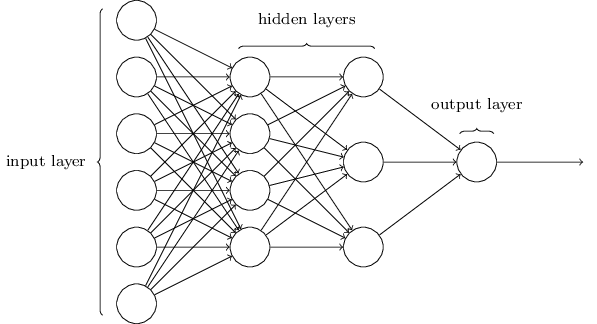
\includegraphics[width=10cm,height=5cm]{NN.jpg}
\caption{Neural Network}
\end{figure}
\\
Since the function is concave in W, the network is expected to get better answers until eventually its performance stops improving. How much the weights are changed is controlled by the learning rate $\nu$. If it is too big, the weights will change a lot  making the network unstable so that it never settles down. On the other hand, if $\nu$ is too short it will be stable and resistant to errors and inaccuracies in the data, but it will take too long to learn. The typical learning rate is between 0.1 and 0.4 \cite{marsland2015machine}.

\section{Hebbian Learning}
Another similar approach is the Hebbian learning proposed by Donald Hebb. He afirmed that the neurons might organize themselves into engrams in the brain. An engram is a memory fragment and it refers to the changes that occur in the brain n response to external stimuli \cite{strom2007hebbian}.

The general idea of the Hebb's basic principle is that any two cells or systems that are repeatedly active at the same time will tend to become 'associated', so that activity in one facilitates activity in the other \cite{morris1999hebb}.

This means that if the firing of one neuron repeatedly leads to the firing of another, the influence of the first on the second increases. Thus increasing the likelihood that the  first will cause the second fire.
It should be notices that the theory refers to neurons which excite neighboring neurons \cite{strom2007hebbian}.
The mathematical expression is as follows:
\begin{equation}
\label{eq:hebbianrule}
w_ij (t+1)= w_ij(t)+\eta x_i(t)x_j(t)
\end{equation}

If $x_i$ and $x_j$ fire then the weight is adjusted. The problem here is that it describes the increasing of weights in a network but without a bound so it is unstable. There are some solutions like setting an upper bound on weights in the network and weight normalization as in the case of the Oja's rule showed as follows \cite{oja1982simplified}:
\begin{equation}
\label{eq:ojasrule}
w_ij (t+1)= w_ij(t)+\eta x_j(t)(x_i(t) - w_ij(t)x_j(t))
\end{equation}
Oja's rule regulates the amount of learning by decreasing the amount of adjustment that occurs as $w_ij$ increases.

\subsection{Hopfield networks}
Hopfield networks are a type of recurrent neural networks that are effective when used as associative memory \cite{hopfield1982neural}. This networks have the property that they may return a pattern similar to the one presented if such a pattern exists n its memory.The activation function is discrete with binary outputs ${-1,+1}$ and the neurons fire when the input accumulation exceeds the threshold of 0. Their connections have two restrictions:
\begin{enumerate}
\item A neuron can not have a connection to itself
\item All connections must be symmetrical meaning if $w_i$ is valid then $w_j$ is too with $w_ij=w_ji$
\end{enumerate}
Training of Hopfield networks is Hebbian. When a pattern is presented to the outputs of the network, the weights in \ref{eq:hopfield} are adjusted following the Hebbian rule and the anti Hebbian rule which is the opposite. Thus, if two neurons have the same value, the weight between them is increased and if they have the opposite value, it is decreased \cite{strom2007hebbian}.
\begin{equation}
\label{eq:hopfield}
E= -\frac{1}{2} \sum_{i<j} w_ij x_i x_j + \sum_i \theta_i x_i
\end{equation}

\section{Deep Learning}
As explained before, learning in the context of artificial neural networks refers to finding the adequate weights that make the network exhibit the desired behavior. Depending on the problem and how the neurons are connected, such behavior may require long causal chains of computational stages, where each stage transforms the aggregate activation of the network. Deep Learning is about accurately assigning credit across many such stages \cite{schmidhuber2015deep}.

Another way of understanding deep learning is by studying neural networks as a representation learning method. This kind of methods allow a machine to be fed with raw data and to automatically discover the representations needed for detection or classification. Hence, deep learning methods are representation learning methods with multiple levels of representation. With the composition of enough transformations, very complex functions can be learned \cite{lecun2015deep}. This work will focus on Recurrent Neural Networks, a subfield of Deep Learning in Artificial Neural Networks (NNs).


\subsection{Recurrent Neural Networks}

A deep recurrent neural network (RNN) is a deep artificial neural network model but with a different structure. In the deep case, connections among hidden units are allowed. Furthermore, these connections are associated with a time delay enabling the model to retain information about the past inputs. In this way, temporal correlations between events that are possibly far away from each other in the data can be discovered \cite{pascanu2013difficulty}.

\begin{figure}
\label{fig:rnn}
\center
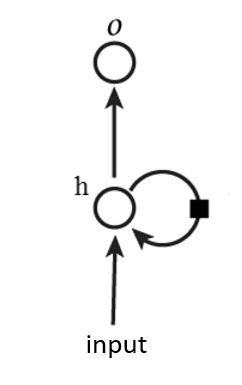
\includegraphics[width=3.5cm,height=5cm]{rnn.png}
\caption{Recurrent Neural Network}
\end{figure}
For tasks that involve sequential inputs it results better to use RNNs. This is mainly because RNNs process an input sequence one element at a time and maintain in their hidden units a "state vector". This vector implicitly contains information about the history of all the past elements of the sequence.\cite{lecun2015deep} 

Although sequential data often arise through measurement of time series such as the rainfall measurements on successive days at a particular location, or the daily values of a currency exchange rate; sequential data can also arise in other contexts such as the sequence of words or characters in a an English sentence \cite{bishop2006pattern}. The order of the elements of a sentence as well as the relationships between them matter. Thus, to predict which is the most likely element to follow the sequence, it is important to retain this information.

In this case the input data is the set of elements of a sentence or a set of sentences and the desired behaviour is to generate a new sequence that can adequately continue after the original one. Therefore, the target data for each element is the following one. The recurrent neural network receives an input vector $x=[x_1,...,x_T]$ which is passed through weighted connections to N recurrently connected hidden vector sequences $h^n=[h_1^n,...,h_T^n]$ and finally to the output vector sequence $y=[y_1,...,y_T]$ which will be compared to the target value for each observation.To compute the hidden layer activation the following equations are iterated from t=1 to T and from n=2 to N. \cite{graves2013generating}:

\begin{equation} \label{eq:hidden1}
h_t^1= H( W_{ih^1} * x_t + W_{h^1 h^1}*h^1_{t-1} + b^1_h)
\end{equation}

\begin{equation} \label{eq:hidden}
h_t^n= H(W_{ih^n} * x_t + W_{h^{n-1}  h^n} * h^{n-1}_t +W_{h^n h^n} * h^n_{t-1}+ b^n_h)
\end{equation}

The W terms denote the weight matrices that connect the input layer to the first hidden layer, two hidden layers between them or a hidden layer to an output layer. $H$ is the hidden layer function which usually is an application of a sigmoid function like the hyperbolic tangent. Finally, given the hidden sequences, the output sequence is computed as follows:

\begin{equation} \label{eq:output}
y_t=Y(\sum_{n=1}^{N} W_{h^{n}y} * h^n_t + b_y)
\end{equation}

Where $Y$ is the output layer function whose output vectors will need to be compared to the target values so that the network achieves the desired behaviour by minimizing the difference between both values. In Equation \ref{eq:error} the error was defined as this difference. Nevertheless, this definition is not adequate given the nature of the data. It is better to use the entropy to compute the loss since it returns a greater value the further it is from the correct target  value. The entropy is the negative logarithm of the predictive distribution as showed in equations \ref{eq:prdist} and \ref{eq:loss}:

\begin{equation} \label{eq:prdist}
P(x)=\Pi_{t=1}^{T} P(x_{t+1}|y_t)
\end{equation}
Finally,the sequence loss is the negative logarithm of \ref{eq:prdist}
\begin{equation} \label{eq:loss}
L(x)=\sum_{t=1}^{T} P(x_{t+1}|y_t)
\end{equation}

The network now can be trained using the gradient descent to know how the parameters should be changed to decrease the loss. Therefore, the partial derivatives of the loss with respect to the weights should be computed. This can be achieved using backpropagation through time.


\subsubsection{Backpropagation Through Time}

The objective here is to understand how the $W$ vector should change to decrease the loss $L(x)$. To achieve this, the gradient of the loss with respect to the weights should be computed using backpropagation through time (BTT). This process computes the gradients of expressions through recursive application of the chain rule. 

BTT applied to RNNs have the constraint of sharing the parameters within each layer. As showed in  \ref{fig:unfold}, RNNs once unfolded in time can be seen as very deep feedforward networks in which all the layers share the same weights\cite{lecun2015deep}. Here, the model is presented as a deep multi-layer one where each time step in the interval $[t,T]$ is a layer with N units each \cite{pascanu2013difficulty}. Hence, the constraint can be satisfied by adding the gradients for W at each time step. Although it is a constraint it can also be seen as an advantage since the network requires less number of parameters than a non-recurrent neural network.

\begin{figure}
\label{fig:unfold}
\center
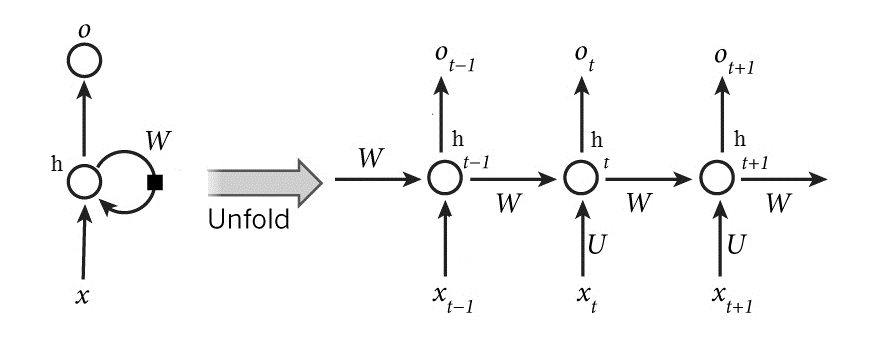
\includegraphics[width=10cm,height=5cm]{unfold.png}
\caption{Unfolded Recurrent Neural Network}
\end{figure}

The key insight in BTT is that the calculation of the derivative of the objective with respect to the input of a module can be done by working backwards from the gradient with respect to the output of that module and repeating this process through all the layers or, in this case, through all the time steps \cite{schmidhuber2015deep}.

\begin{figure}
\label{fig:bpt}
\center
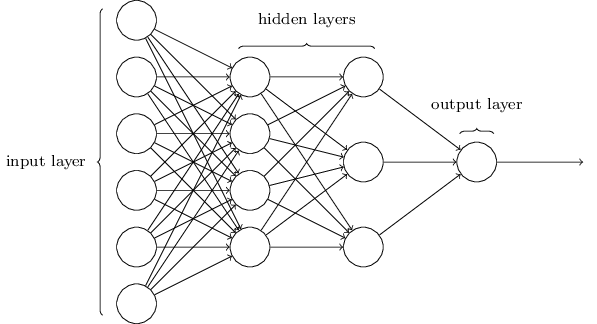
\includegraphics[width=10cm,height=5cm]{NN.jpg}
\caption{Neural Network}
\end{figure}
%a lo mejor aquí poner lo del -1

\subsubsection{RNNs Training Issues}
As described before, RNNs are very powerful dynamic systems. Unfortunately training them has proved to be problematic. During the gradient backpropagation phase, the gradient signal can end up being multiplied a large number of times by the weight matrix associated with the connections between the neurons of the recurrent hidden layer. This causes that the backpropagated gradients either grow or shrink at each time step. Thus, the magnitude of weights in the transition matrix may have a strong impact on the learning process.

If the  weight matrix is smaller than 1, the gradient signal can get so small that so over many time steps it can vanish. Conversely, if the eigenvalue of the weight matrix is larger than 1, it can lead to a situation where the gradient signal is so large that it can explode causing learning to diverge. 

The exploding gradients problem refers to the large increase in the norm of the gradient during training caused by the explosion of the long term components. On the other hand, the vanishing gradients problem is presented when long term components go exponentially fast to norm 0 making impossible for the model to learn correlation between temporally distant events \cite{pascanu2013difficulty} which was the main reason for choosing RNNs for this work. 

\subsubsection*{The exploding gradients problem}
 The fact that the norm of the gradient increases during training is a problem because the computation becomes inefficient and it increases the response time. One simple mechanism to deal with this problem is to rescale them whenever they go over a threshold. To choose wisely the threshold, one good heuristic is to look at statistics on the average norm over a sufficiently large number of updates. In this way, we can handle very abrupt changes in norm. In this case, the algorithm can be thought of as adapting the learning rate based on the norm of the gradient  \cite{pascanu2013difficulty}.
%Poner en cuánto se fija 

\subsubsection*{The vanishing gradients problem}

The vanshing gradients problem makes it difficult to learn to store information for very long and this amnesia makes them prone to instability when generating sequences. The main problem is that if the network's predictions  are only based on the last few inputs, and these inputs were themselves predicted by the network, it has little opportunity to recover from past mistakes.

On the other hand, having a longer memory has a establishing effect, because even if the network cannot make sense of its recent history, it can look further back in the past to formulate its predictions. \cite{graves2013generating}

A lot of research work has been made to propose solutions to this problem. The idea is to augment the network with an explicit memory. The first proposal of this kind is the long short-term memory (LSTM) network used in this work. The LSTM has complicated dynamics that allow it to easily “memorize” information for an extended number of timesteps \cite{zaremba2014recurrent}.


\subsubsection{Long Short-Term Memory Networks}
Long Short-term Memory (LSTM) is an RNN architecture. The difference is that instead of using a sigmoid function as hidden layer function, LSTMs use memory cells to store information. The new arquitecture has three gates and a memory cell. The gates are for input , forget, and output functions. The memory cell has a connection to itself at the next time step with a weight of one, meaning it copies its own real-valued state and accumulates the external signal\cite{lecun2015deep}. Thus, it can decide to overwrite the memory cell, retrieve it, or keep it for the next time step\cite{zaremba2014recurrent}. 

LSTMs are better at storing and accessing information than standard RNNs, since the cells improve the performance when finding and exploiting long range dependencies in the data. Additionally, the full gradient can be calculated with backpropagation through time.\cite{graves2013generating}

\begin{figure}
\label{fig:lstm}
\center
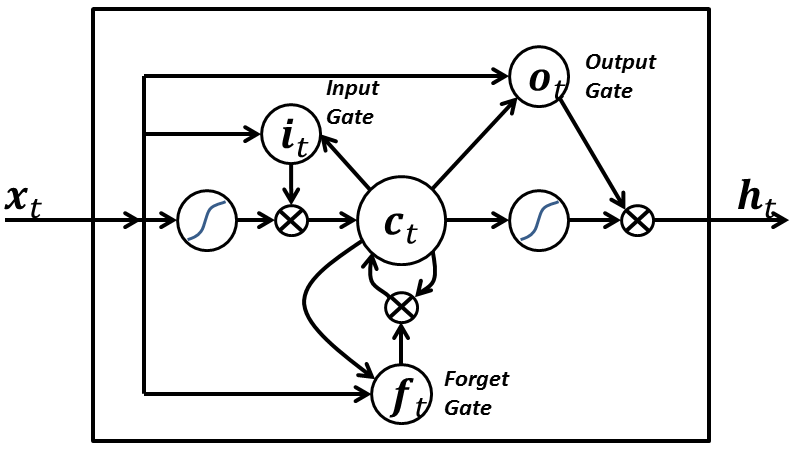
\includegraphics[width=10cm,height=5cm]{Long_Short_Term_Memory.png}
\caption{Long Short Term Memory Network}
\end{figure}

The forget gate $f_t$ decides the content to keep for each time step $t$. It is a sigmoid function that takes in account the $h_{t-1}$ and the present input $x_t$ and returns a number between 0 and 1 where 0 means "forget it" and 1 means "keep it". 

The next step is to calculate the input gate to decide which values to update using a sigmoid function (Eq. \ref{eq:input}). Then, the new candidates are computed by a tanh function (Eq. \ref{eq:candidate}), and the memory cell update is done by combining the previous functions as explained in Eq. \ref{eq:update}.

\begin{equation} \label{eq:forget}
f_t=\sigma(W_f*(h_{t-1},x_t)+b_f)
\end{equation}
\begin{equation} \label{eq:input}
i_t=\sigma(W_i*(h_{t-1},x_t)+b_i)
\end{equation}
\begin{equation} \label{eq:candidate}
C'_t=tanh(W_C*(h_{t-1},x_t)+b_C)
\end{equation}
\begin{equation} \label{eq:update}
C_t=f_t*C_{t-1}+i_t*C'_t
\end{equation}

Finally, the output function decides which parts of the memory cell to return with another sigmoid function (Eq. \ref{eq:output}), and lastly the $h_t$ is calculated (Eq. \ref{eq:hidden}) with the output function and a tanh function of the memory cell to push the values into the interval [-1,1].

\begin{equation} \label{eq:output}
o_t=\sigma(W_o*(h_{t-1},x_t)+b_o)
\end{equation}
\begin{equation} \label{eq:hidden}
h_t=o_t*tanh(C_t)
\end{equation}

\subsection{Regularization}

Successful applications of neural networks require good regularization. Although deep neural nets with a huge number of parameters are very powerful machine learning systems they tend to overfit at training time. Combining many different large neural nets at test time is not an efficient solution to address this problem since large networks are also slow to use. 

Fortunately, dropout is a technique for addressing this problem. The key idea is to randomly drop units (along with their connections) from a neural network during training in order to prevent the units from co-adapting too much \cite{srivastava2013improving}. However, when working with recurrent neural networks and specifically with LSTM networks it is not desired to erase all the information from the units. It is extremely important that the units remember events that occurred many timesteps in the past. This is the reason for \cite{zaremba2014recurrent} to only use drop out in the non-recurrent connections. 

Nevertheless, in \cite{gal2015theoretically} they develop a technique to effectively use drop out in all connections in a RNN: Variational RNN. In this dropout variant, the same dropout mask at each time step is repeated for both inputs, outputs, and recurrent layers, meaning that the same network units are dropped at each time step. The interpretation for this work (character-level language modelling) is to force the model not to rely on single characters for its task. In the same work they found that the optimal dropout
probabilities are between 0.3 and 0.5.

\subsection{Gradient Descent Variants}
As previously Gradient Descent is a an optimization algorithm used to find the parameters that minimize an objective function
There are three variants of the gradient descent: batch gradient descent, stochastic gradient descent, and mini-batch gradient descent. The variants differ in how much data is used to compute the gradient of the objective function. 

The first variant computes the gradient of the cost function with respect to the parameters($\theta$) for the entire dataset as in \ref{eq:batchgd}.

\begin{equation} \label{eq:batchgd}
\theta=\theta+\eta * \Delta_\theta * J(\theta)
\end{equation}

The second variant computes a parameter update for each training example $x_i$ and target $y_i$ \ref{eq:sgd}.
\begin{equation} \label{eq:sgd}
\theta=\theta+\eta * \Delta_\theta; * J(\theta;x_i;y_i)
\end{equation}

Were $\eta$ is the learning rate.

The problem with the batch gradient descent is that it can be very slow and it does not allow to update the model with new examples on-the-fly. The stochastic gradient descent solves this problem and is faster than the batch gradient descent, but it performs updates with high variance causing the objective function to fluctuate heavily.  

Finally, the mini-batch gradient descent performs an update for every mini-batch of $n$ training examples as in \ref{eq:mbgd} \begin{equation} \label{eq:mbgd}
\theta=\theta+\eta * \Delta_\theta * J(\theta;x_{i:i+n};y_{i:i+n})
\end{equation}

In this way, the mini-batch gradient descent reduces the variance of the updates, is faster than the first variant and allow the model to update with examples on-the- fly. Therefore, this third option is the chosen one for this work\cite{ruder2016overview}. 


\subsection{Gradient Descent Optimization Algorithms}
To our knowledge, mini-batch Gradient Descent (SGD) is the best option to find the parameters that minimize an objective function. Mini-batch gradient descent is stochastic since the objective function is composed of a sum of subfunctions evaluated at different subsamples of data. Another source of noise may also come inherent function noise and from dropout regularization \cite{kingma2014adam}. 

Choosing the proper learning rate $\eta$ is a difficult and important task as explained in the section "Neural Networks". There is a lot of research around this topic. In \cite{robbins1951stochastic} they try to adjust the learning rate by reducing the learning rate according to a pre-defined schedule or when the change in the objective between epochs falls below a threshold. Another issue is that the same learning rate for all parameter updates may not be the best choice if the data is sparse and the features have different frequencies. In this case, it would be better to perform a larger update for rarely occuring features. One last challenge is to avoid getting trapped in a local minima when working with non-convex objective functions as is the usual case in deep learning. For this cases, efficient stochastic techniques as the ones explained in the following are required \cite{ruder2016overview}.
%fuente:http://sebastianruder.com/optimizing-gradient-descent/
The main algorithms used to avoid those challenges in deep learning applications are: Momentum, Nesterov and the accelerated gradient, Adagrad, RMSPop, and Adam.

Momentum \cite{qian1999momentum} is a method that helps accelerate gradient descent in the relevant direction and dampens oscillations by taking in account a fraction $\phi$ of the update vector of the past time step to the current update vector:

\begin{equation}
\theta=\theta-(\nu_t=\phi \nu_{t-1} + \eta \Delta_\theta J(\theta))
\end{equation}
Where $\phi$ is the momentum term usually set to 0.9.

%The momentum term increases for dimensions whose gradients point in the same directions and reduces updates for dimensions whose gradients change directions. As a result, we gain faster convergence and reduced oscillation.
%chance y quitar esto

Nesterov accelerated gradient \cite{nesterov1983method} not only uses the momentum term $\phi \nu_{t-1}$  to move the parameters $\theta$; but it also computes $\theta - \phi \nu_{t-1}$ to give an approximation of the next position of the parameters.  
\begin{equation}
\theta=\theta-(\nu_t = \phi \nu_{t-1} + \eta \Delta_\theta J(\theta - \phi \nu_{t-1})
\end{equation}

\subsubsection{Adagrad}
\subsubsection{RMSProp}
\subsubsection{Adam}
The name Adam comes from adaptive moment estimation. It combines the advantages of AdaGrad and RMSProp. 

\section{Language Modelling}
There are a lot of technology applications for language modelling. For example, speech recognition, machine translation, document classification and routing, optical character recognition, information retrieval, handwriting recognition, spelling correction, and many more.

Language modelling, also refered as text prediction is possible by generating novel sequences from a trained network assuming the predictions are probabilistic. To achieve this task, samples from the network's output distribution must be generated and then the sample is used as input at the next step. In this way the network treats its inventions as if they were real \cite{graves2013generating}.

\subsection{Text Representation}
Text data is discrete, and is typically represented using one-of-k representation also called one-hot representation. This consists of input vectors of the same length as the number of text classes $K$. Each entry of the vector fed in a time $t$ and belonging to class $k$ is zero except for the $kth$, which is one. The predictive distribution function in equation \ref{eq:prdist} is therefore a multinomial distribution, which can be parameterised by a softmax function at the output layer as follows \cite{graves2013generating}:

\begin{equation} \label{eq:multinomial}
P(x_{t+1}=k|y_t)=y^k_t=\frac{\mathrm{e}^{Y^k_t}}{ \sum_{k=1}^{K} \mathrm{e}^{Y^k_t}}
\end{equation}

The fact that equation \ref{eq:multinomial} is multinomial implies that unlike the distribution function \ref{eq:prdist}, there is more than one result,$K$ in this case, one for each text class.  It turns the output into a probability distribution over the categories making the values of the network outputs sum to 1. Thus, the network indicates the probability for each character to be the next one.

The categorical cross-entropy loss the standard loss function for multilabel classification, which basically penalizes the network more the further off it is from the correct label. The next step is to express the loss function for equation \ref{eq:multinomial}. Substituing it into the original entropy function \ref{eq:loss} it expresses the cross entropy as follows \cite{graves2013generating}:

\begin{equation} \label{eq:crossEntropy}
L(x)=-y \sum_{t=1}^{T} log y^{x_t+1}_t
\end{equation}

Finally, the derivative of \ref{eq:crossEntropy} after using the chain rule to derive the gradient, and after cancelling out a lot of terms, turns out to be a simple and interpretible expression as showed in Eq. \ref{eq:gradient}.

\begin{equation} \label{eq:cgradient}
\frac{\delta L(x)}{\delta Y^k_t}=- y^k_t - 1 (y_t=k)
\end{equation}

When it is not the correct text class $(y_t \not= k)$ the values will be positive, meaning that increasing this score would cause an increased loss. On the other hand, when it is the correct class $(y_t = k)$, the sign will be negative, meaning that increasing this score would reduce the loss.


The last decision that must be made is about choosing the text classes. This is directly related with the level of language modelling that can be either word-level or character-level.

\subsubsection{Word-level language modelling}

In most cases, text prediction is performed at the word level. The number of text classes $K$ is therefore the number of words in the dictionary \cite{graves2013generating}.

In the first layer, each word creates word vectors and the other ones learn to convert the input word vectors into an output word vector for the predicted next word used to predict the probability for any word in the vocabulary. 

Learning word vectors turned out to work very well when the word sequences come from a large corpus of real text. However, for realistic tasks, where the number of words often exceeds 100,000, this can be rather problematic \cite{lecun2015deep}. 
%se tendría que hacer mayor minado pues dos palabras escritas de diferente manera pe por ortografía serían dos diferentes 

Word-level language modelling has several limitations. Having so many classes demands a huge amount of training data to adequately cover the possible contexts for the words. Furthermore, word-level models are not applicable to text data containing non-word strings, such as multi-digit numbers or web addresses.\cite{graves2013generating}

\subsubsection{Character-level language modelling}


Character-level language modelling has been found to give slightly worse performance than equivalent word-level models. Nonetheless, predicting one character at a time is more interesting from the perspective of sequence generation, because it allows the network to invent novel words and strings \cite{graves2013generating}. 

This language modelling option overcomes the great class number limitations of word-level language modelling. In this case, the predictions are not limited to the vocabulary words and it is applicable to text data containing non-word strings. Here, the number of text classes $K$ is defined by the number of different characters in the training data. It also overcomes the language limitation, meaning that the input data can be indifferently in Spanish, English, Chinese, etc.. 

For these reasons character-level modelling is the one chosen for this work.

 




	% \include{Chapters/relatedwork}

	% \include{Chapters/method}

	% \include{Chapters/results}

	% \include{Chapters/conclusions}

	%%%%%%%%%%%%%%%%%%%%%%%%%%%%%%%%%%%%%%%%%%%%%%
	% APPENDIX
	%%%%%%%%%%%%%%%%%%%%%%%%%%%%%%%%%%%%%%%%%%%%%%
	\appendix
	% \include{Chapters/appendixA}

	%%%%%%%%%%%%%%%%%%%%%%%%%%%%%%%%%%%%%%%%%%%%%%
	% BIBLIOGRAPHY
	%%%%%%%%%%%%%%%%%%%%%%%%%%%%%%%%%%%%%%%%%%%%%%
	\clearpage
	\addcontentsline{toc}{chapter}{References} %Añadimos la bibliografia a la lista de contenidos.
	
	%%%%%%%%% Referencias usando el sistema embedido %%%%%%%%%%%
	% e.g. (Ejemplo tomado de https://en.wikibooks.org/wiki/LaTeX/Bibliography_Management)
	%
	% \begin{thebibliography}{9}
	%
	%	\bibitem{lamport94}
    %			Leslie Lamport,
    %			\emph{LaTeX: a document preparation system},
    %			Addison Wesley, Massachusetts,
  	%			2nd edition,
    % 			1994.
    %
	% \end{thebibliography}

	%%%%%%%%% Referencias usando bibtex %%%%%%%%%%%
	\bibliographystyle{plain}
	\bibliography{references} 

\end{document}